%!TEX root = ../template.tex
%%%%%%%%%%%%%%%%%%%%%%%%%%%%%%%%%%%%%%%%%%%%%%%%%%%%%%%%%%%%%%%%%%%%
%% 4-Work_Done.tex
%% NOVA thesis document file
%%
%% Chapter with the template manual
%%%%%%%%%%%%%%%%%%%%%%%%%%%%%%%%%%%%%%%%%%%%%%%%%%%%%%%%%%%%%%%%%%%%

\typeout{NT FILE 5-Decentralized_Development.tex}%

\chapter{Decentralized Development}
\label{cha:Decentralized Development}

\glsresetall

\section{Introduction} \label{sec.5:Introduction}

This chapter focuses on the decentralized implementation of an encirclement algorithm, building heavily on the architecture introduced in Chapter~\ref{cha:Centralized Development}. The main difference in this implementation is that it is no longer possible to determine the desired final positions without prior knowledge of the number of agents. Furthermore, applying the Munkres algorithm, as done previously, would require each agent to have access to the positions of all other agents, which contradicts the principles of a decentralized approach.

As in the previous chapter, this chapter is divided into two main sections: the distribution of points on the two-sphere, and the control architecture responsible for safely guiding agents from arbitrary positions in $\mathbb{R}^3$ to their assigned positions on the two-sphere.

\section{Comparison of Agent Distributions on the Two-Sphere} \label{sec.5:Comparison of Agent Distributions on the Two-Sphere}

As outlined in Section~\ref{sec.3:Iterative computation agent spacing on the two-sphere}, multiple approaches exist for distributing points on the two-sphere, allowing for the total number of agents to be unknown, vary in time, and work under a non fully connected implementation. In this section, the outcomes of each method is presented and systematically compared. Based on this comparison, the most suitable  method is identified in light of the objectives and constraints.

\begin{figure}[htbp]
\centering
\begin{minipage}{0.12\textwidth}
Thomson\\Minimal Energy:
\end{minipage}%
\begin{minipage}{0.85\textwidth}
\subfloat[Normal]{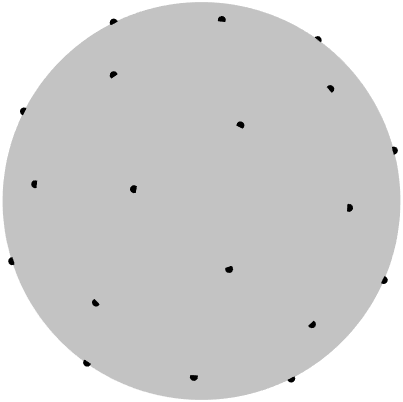
\includegraphics[width=3cm]{5-Figures/Chapter4/thomson_sphere/thomson_normal.png}}\hfil   
\subfloat[Top]{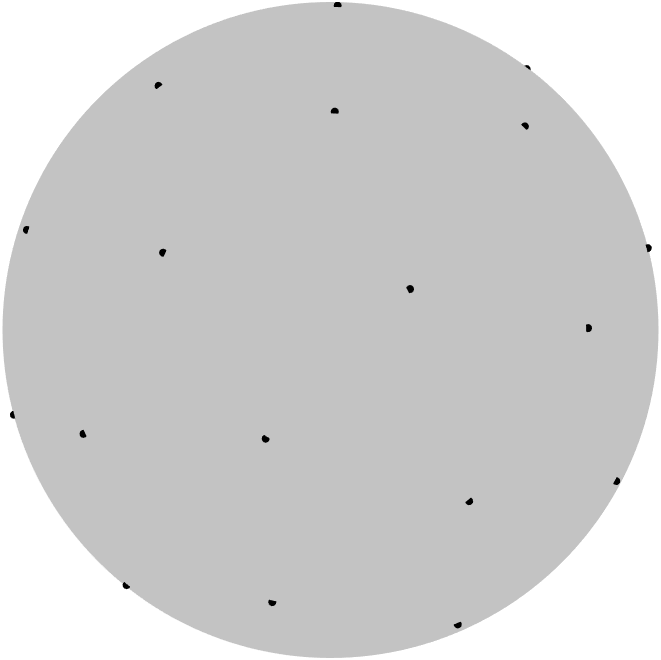
\includegraphics[width=3cm]{5-Figures/Chapter4/thomson_sphere/thomson_top.png}}\hfil
\subfloat[Side]{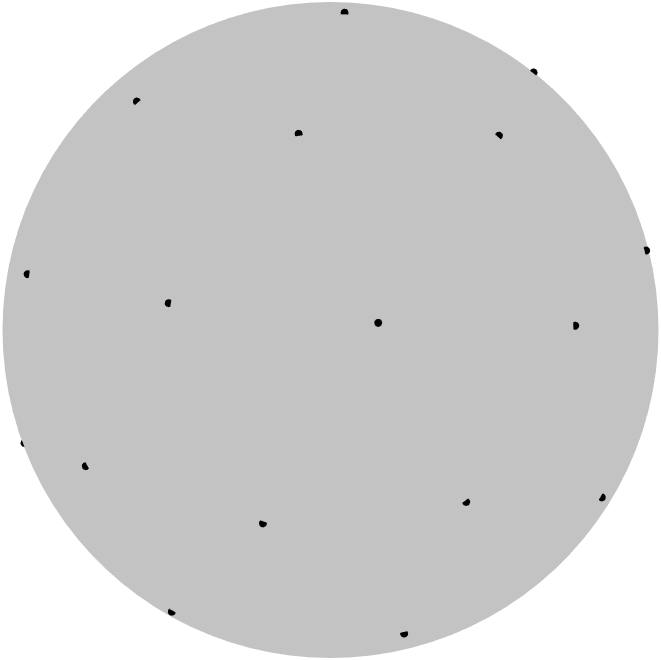
\includegraphics[width=3cm]{5-Figures/Chapter4/thomson_sphere/thomson_side.png}}
\end{minipage}

\vspace{0.3cm}

\begin{minipage}{0.12\textwidth}
Lloyd's\\Algorithm\\
(convex hull):
\end{minipage}%
  \begin{minipage}{0.85\textwidth}
  \subfloat[Normal]{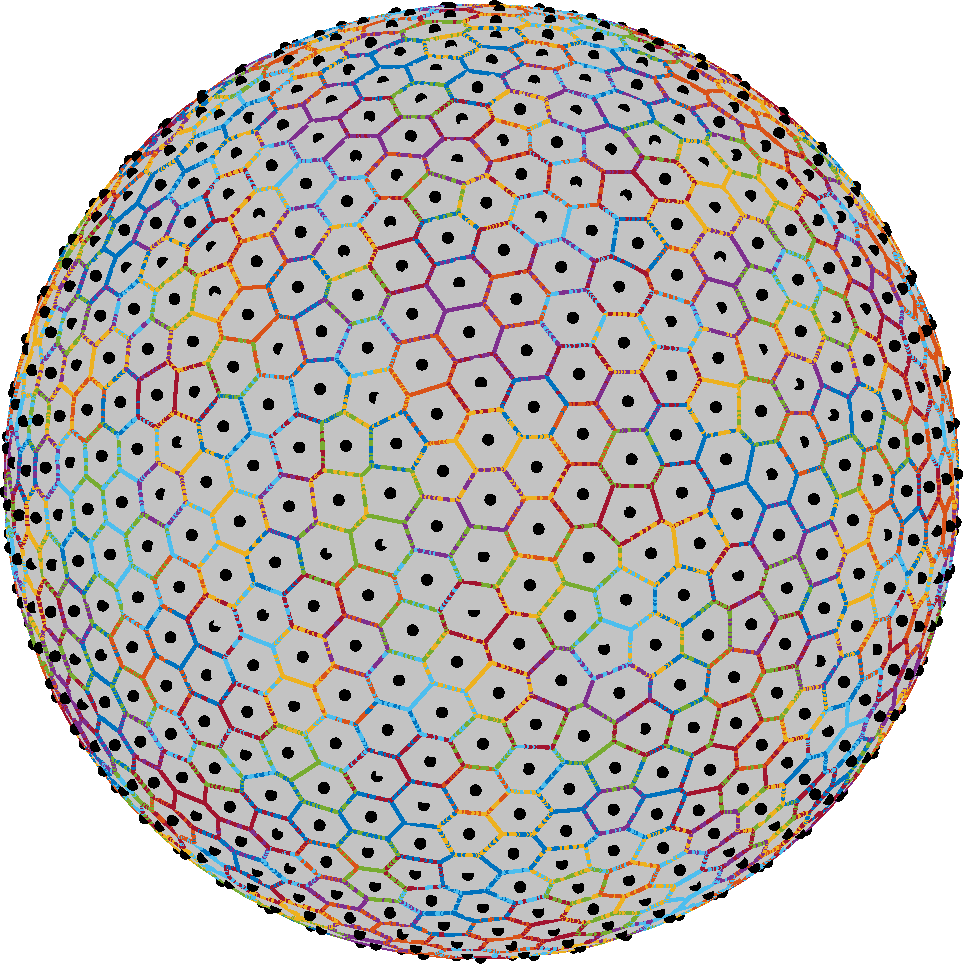
\includegraphics[width=3cm]{5-Figures/Chapter3/Lloyd_convex_hull/Lloyd_normal.pdf}}\hfil   
  \subfloat[Top]{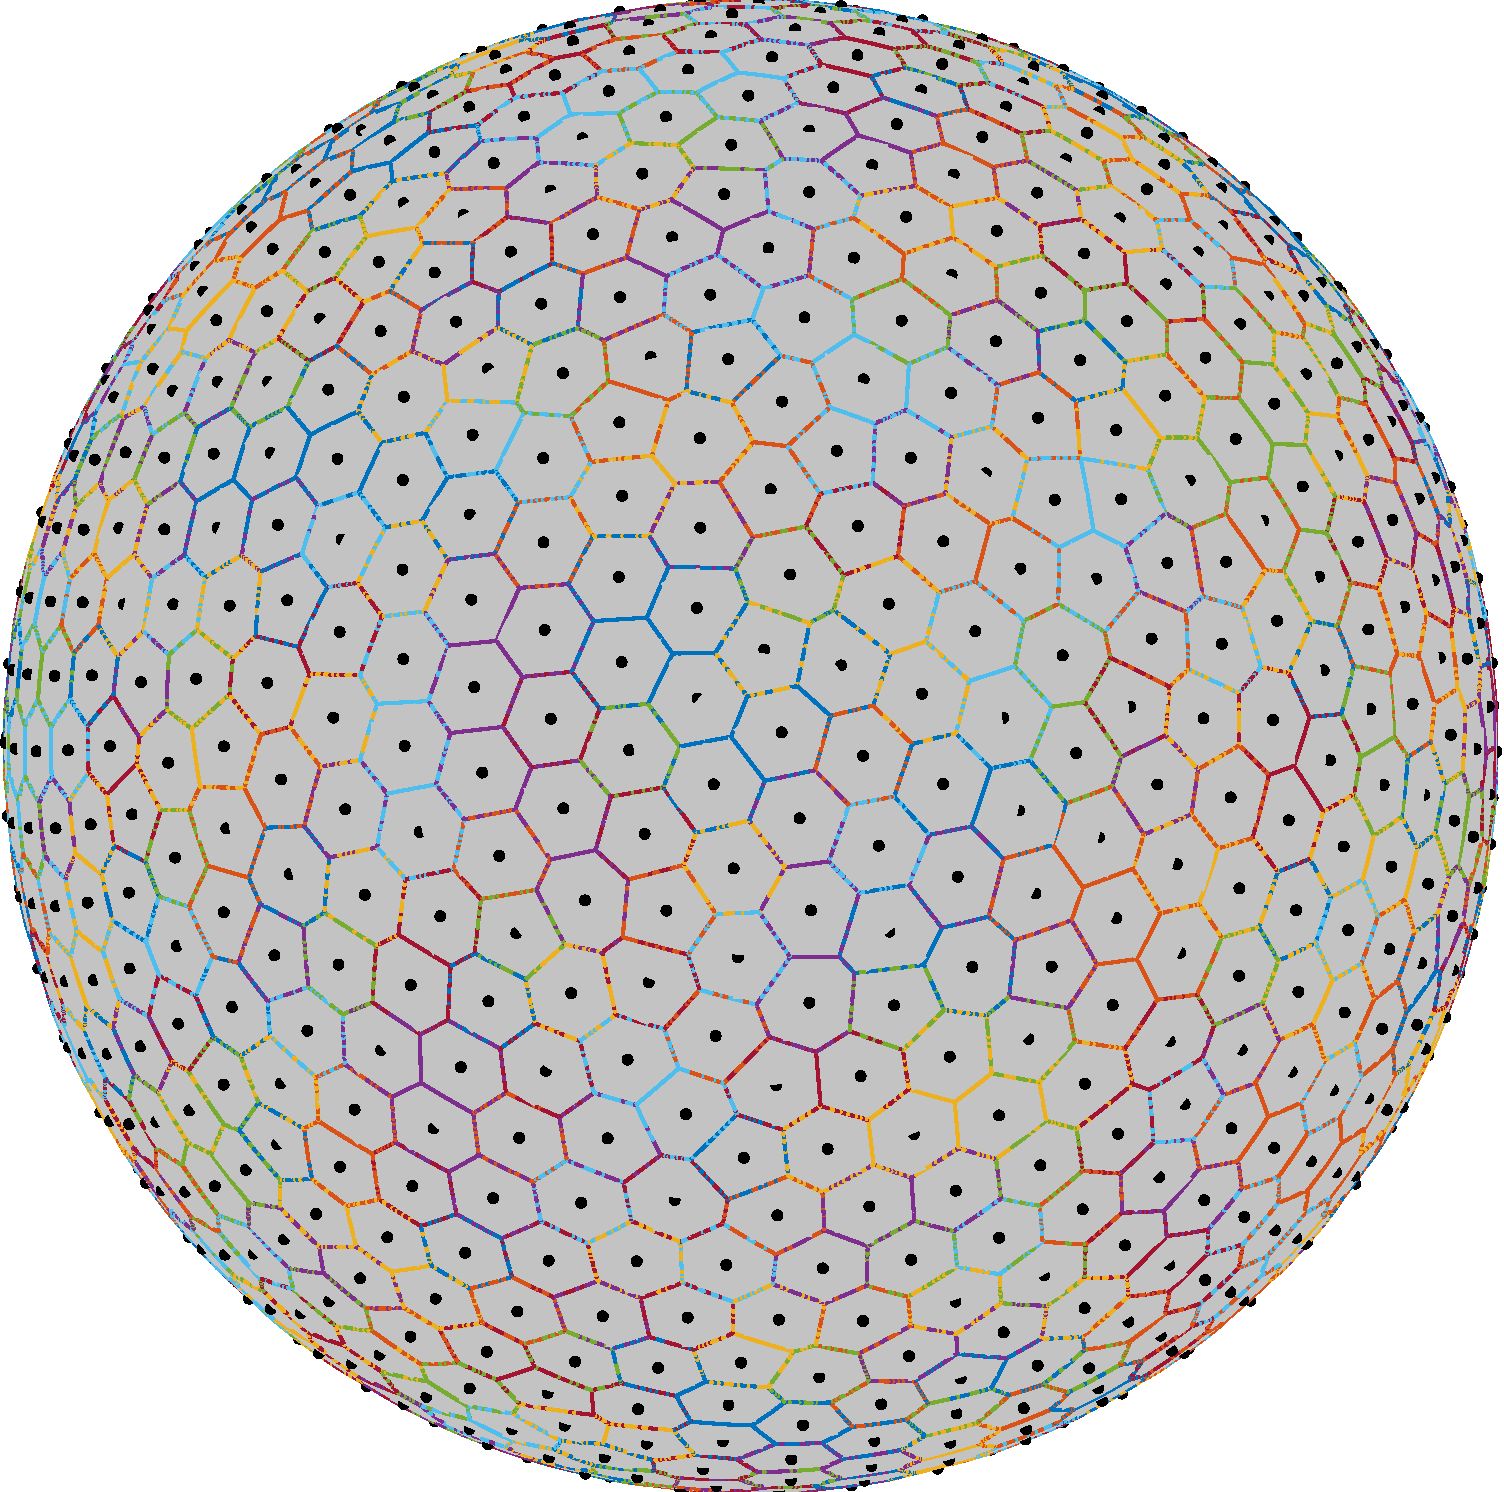
\includegraphics[width=3cm]{5-Figures/Chapter3/Lloyd_convex_hull/Lloyd_top.pdf}}\hfil
  \subfloat[Side]{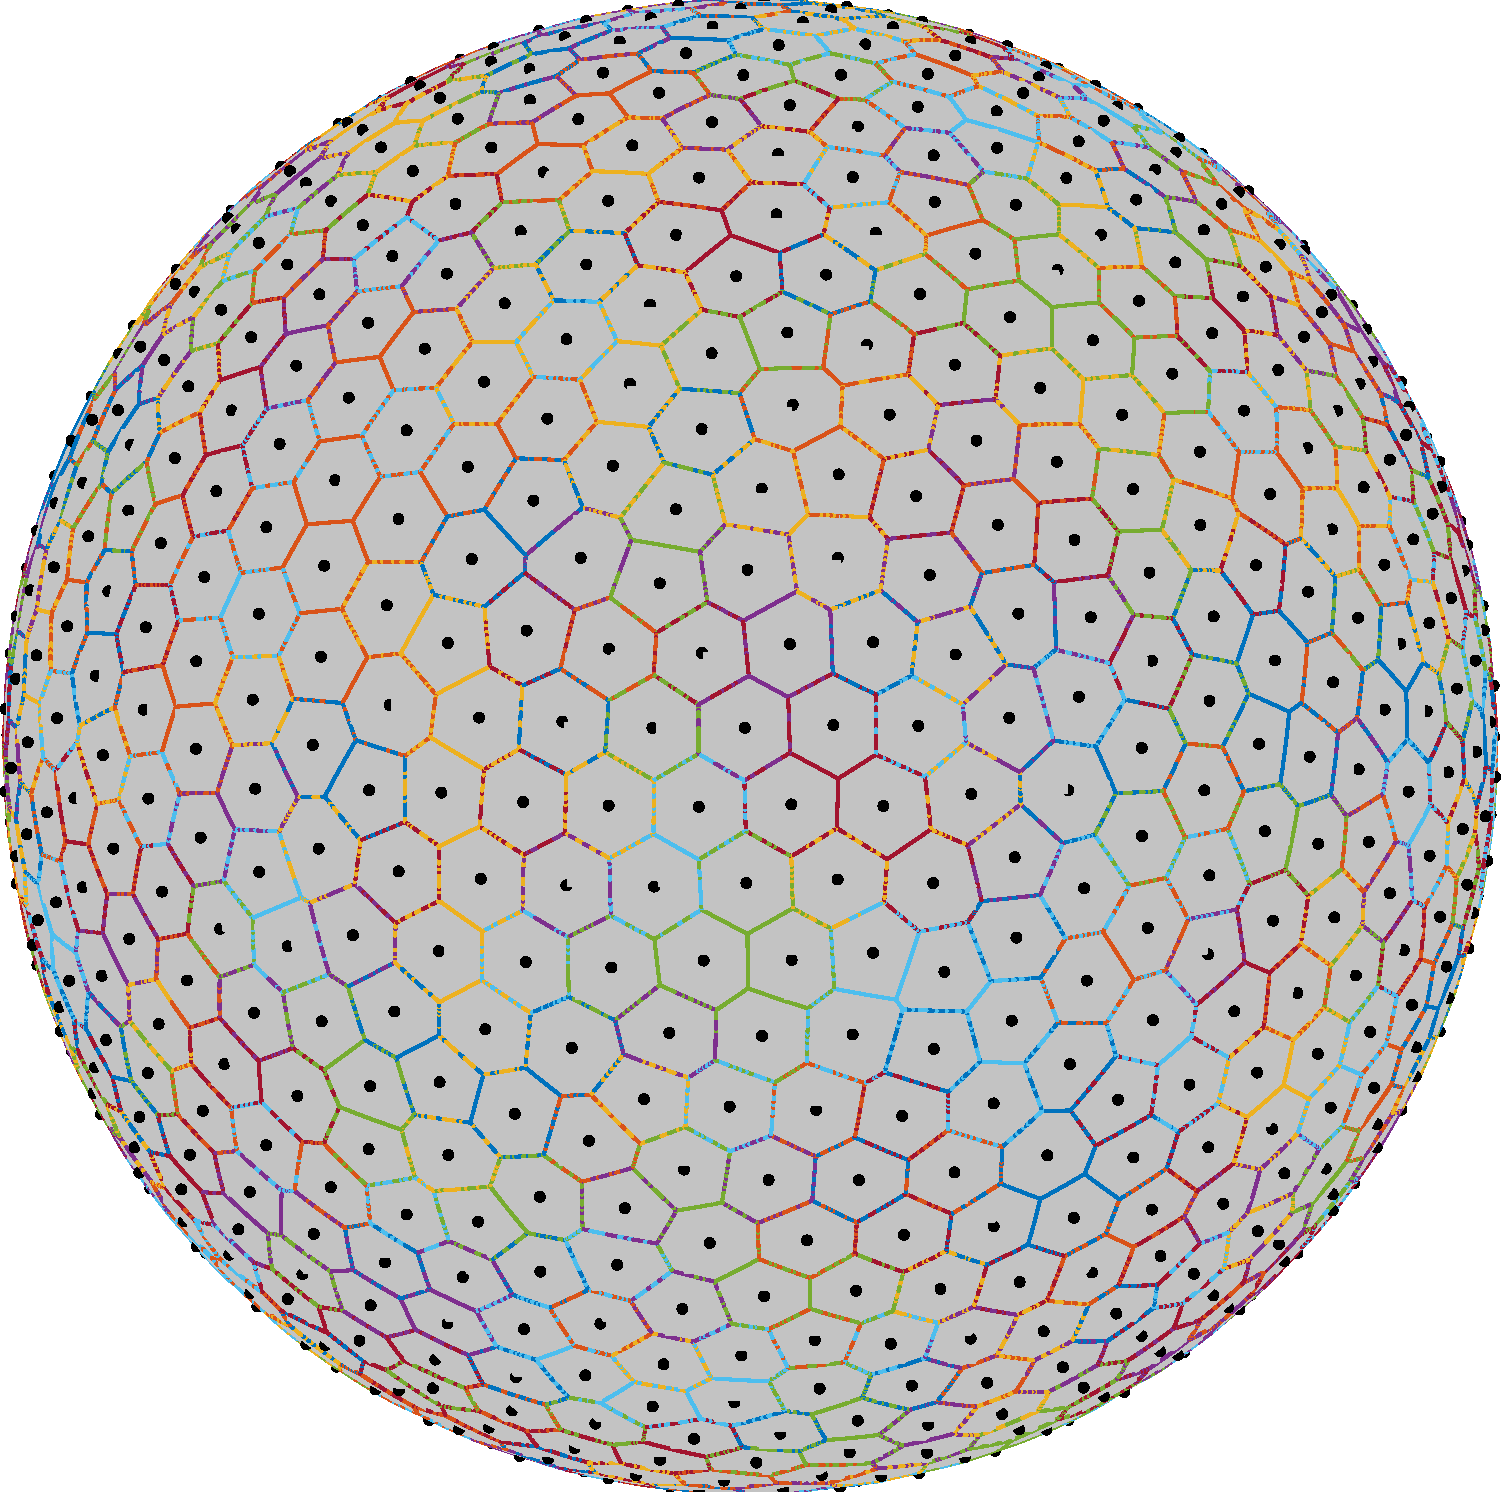
\includegraphics[width=3cm]{5-Figures/Chapter3/Lloyd_convex_hull/Lloyd_side.pdf}}
\end{minipage}

\begin{minipage}{0.12\textwidth}
Lloyd's\\Algorithm\\
(half plane):
\end{minipage}%
  \begin{minipage}{0.85\textwidth}
  \subfloat[Normal]{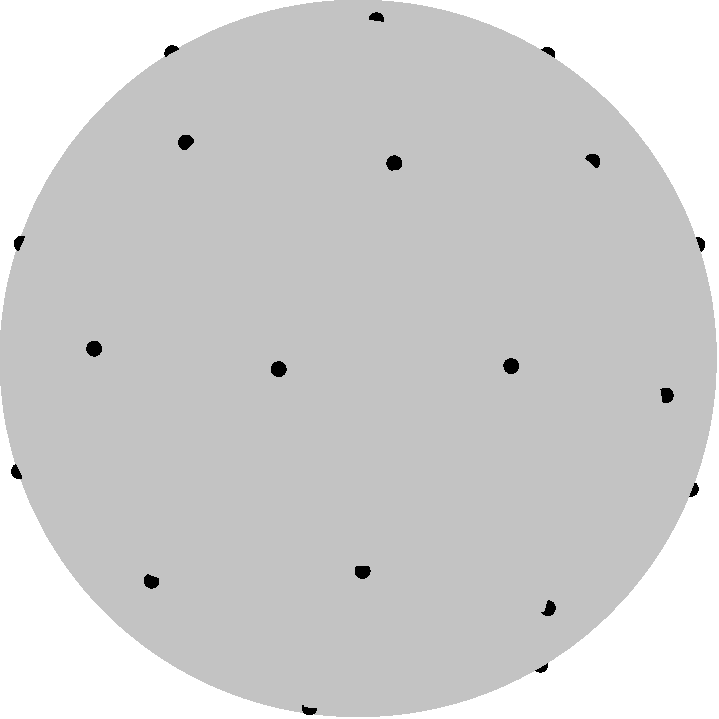
\includegraphics[width=3cm]{5-Figures/Chapter3/Lloyd_half_plane/Lloyd_half_plane_normal.pdf}}\hfil   
  \subfloat[Top]{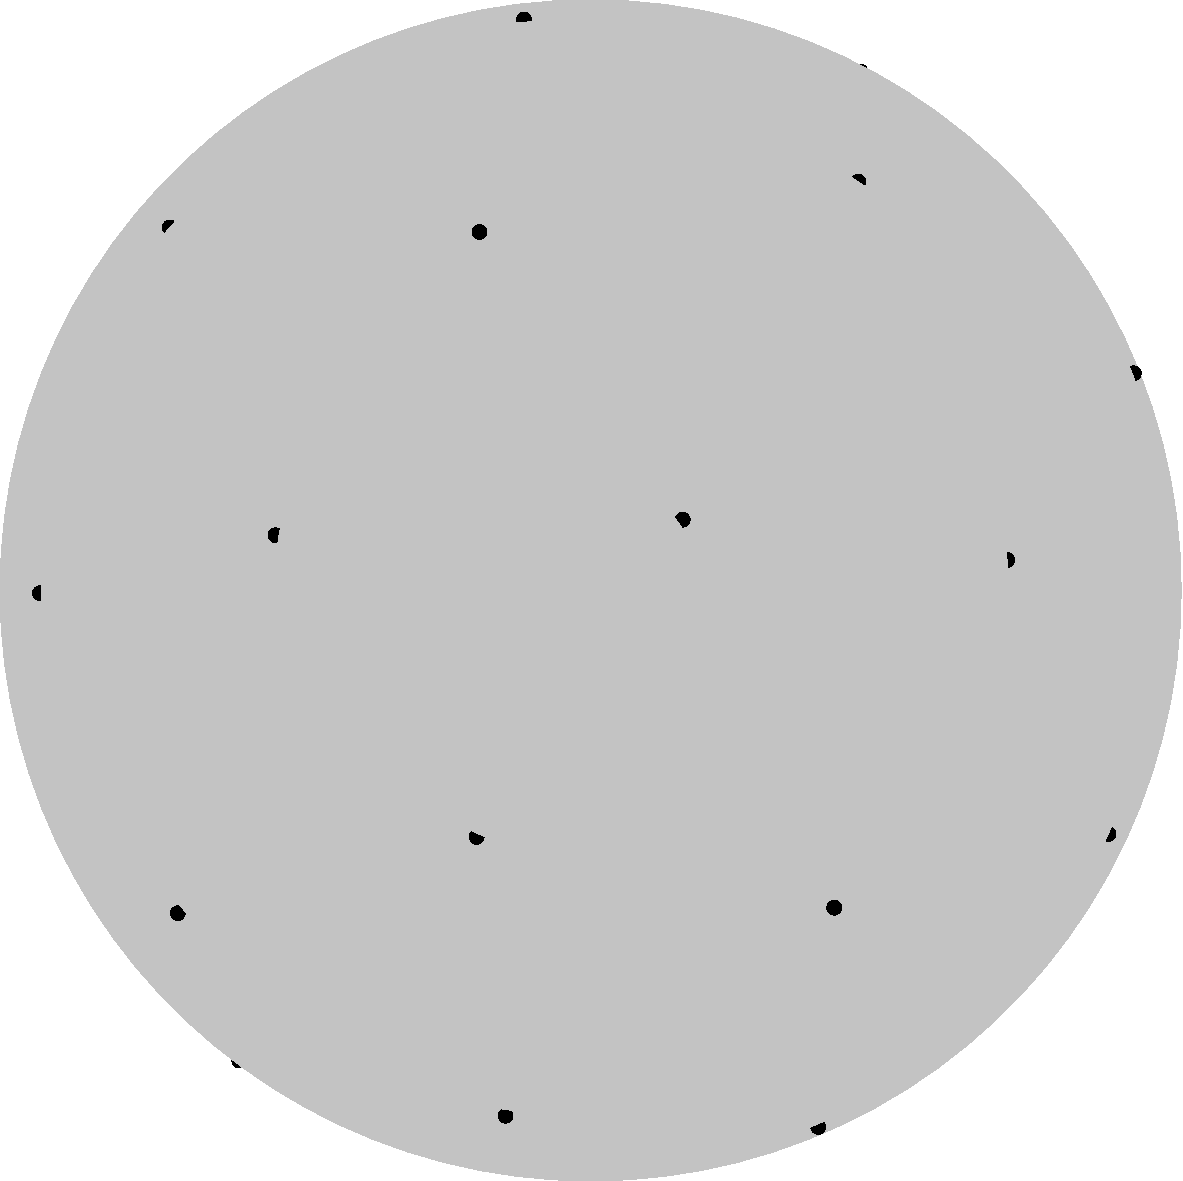
\includegraphics[width=3cm]{5-Figures/Chapter3/Lloyd_half_plane/Lloyd_half_plane_top.pdf}}\hfil
  \subfloat[Side]{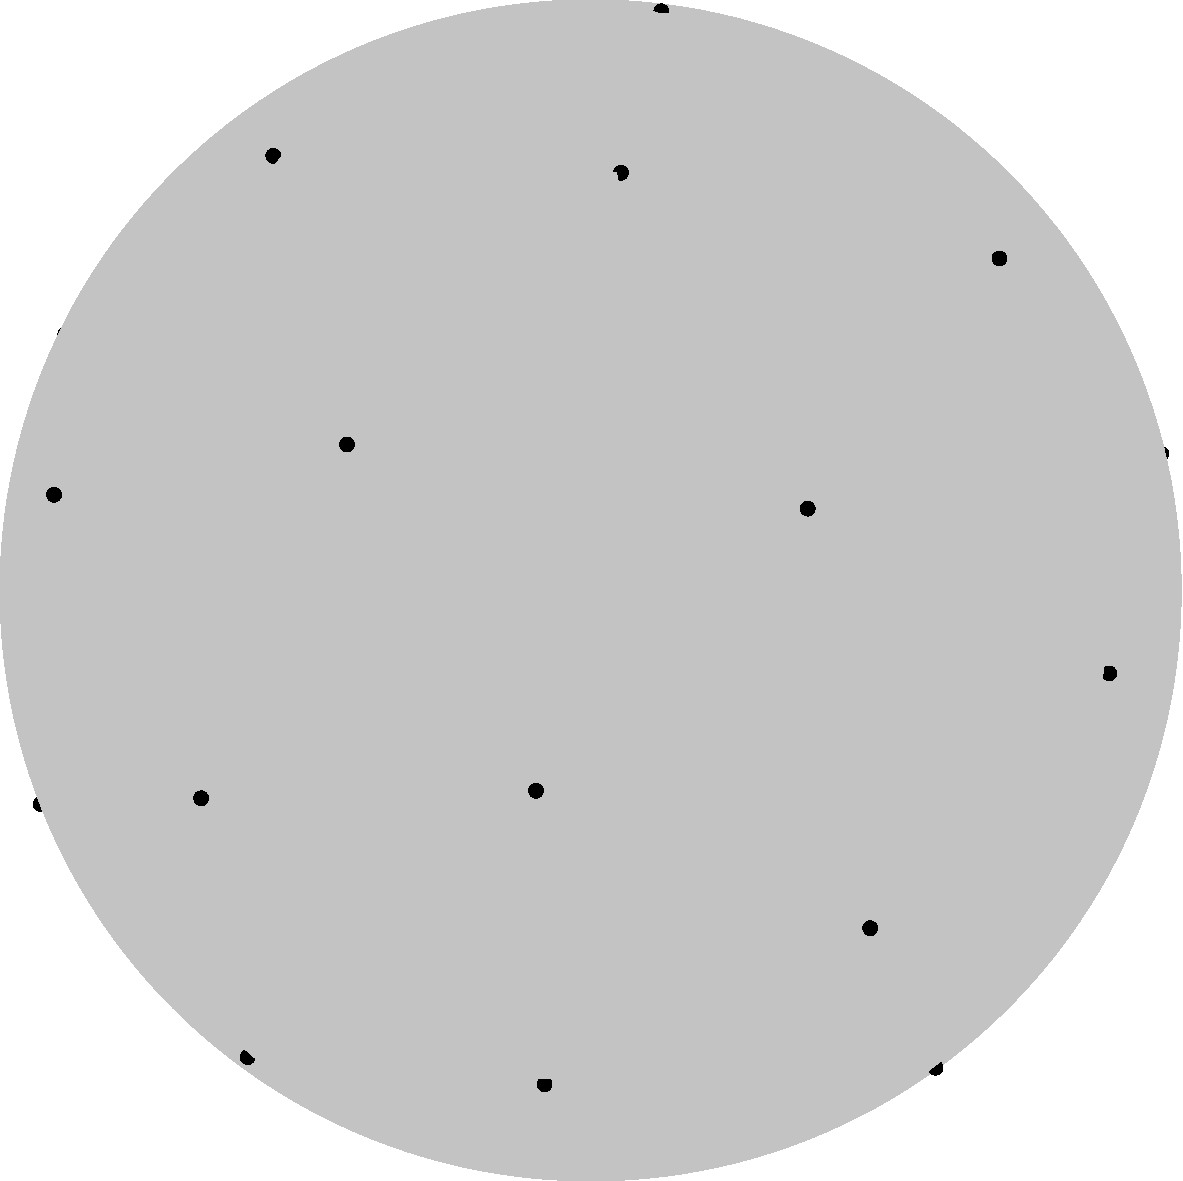
\includegraphics[width=3cm]{5-Figures/Chapter3/Lloyd_half_plane/Lloyd_half_plane_side.pdf}}
\end{minipage}

\caption{Agent positions resulting from each distribution methods.}
\label{fig.5:methods_points_on_sphere}
\end{figure}

\begin{figure}[htbp]
  \centering
  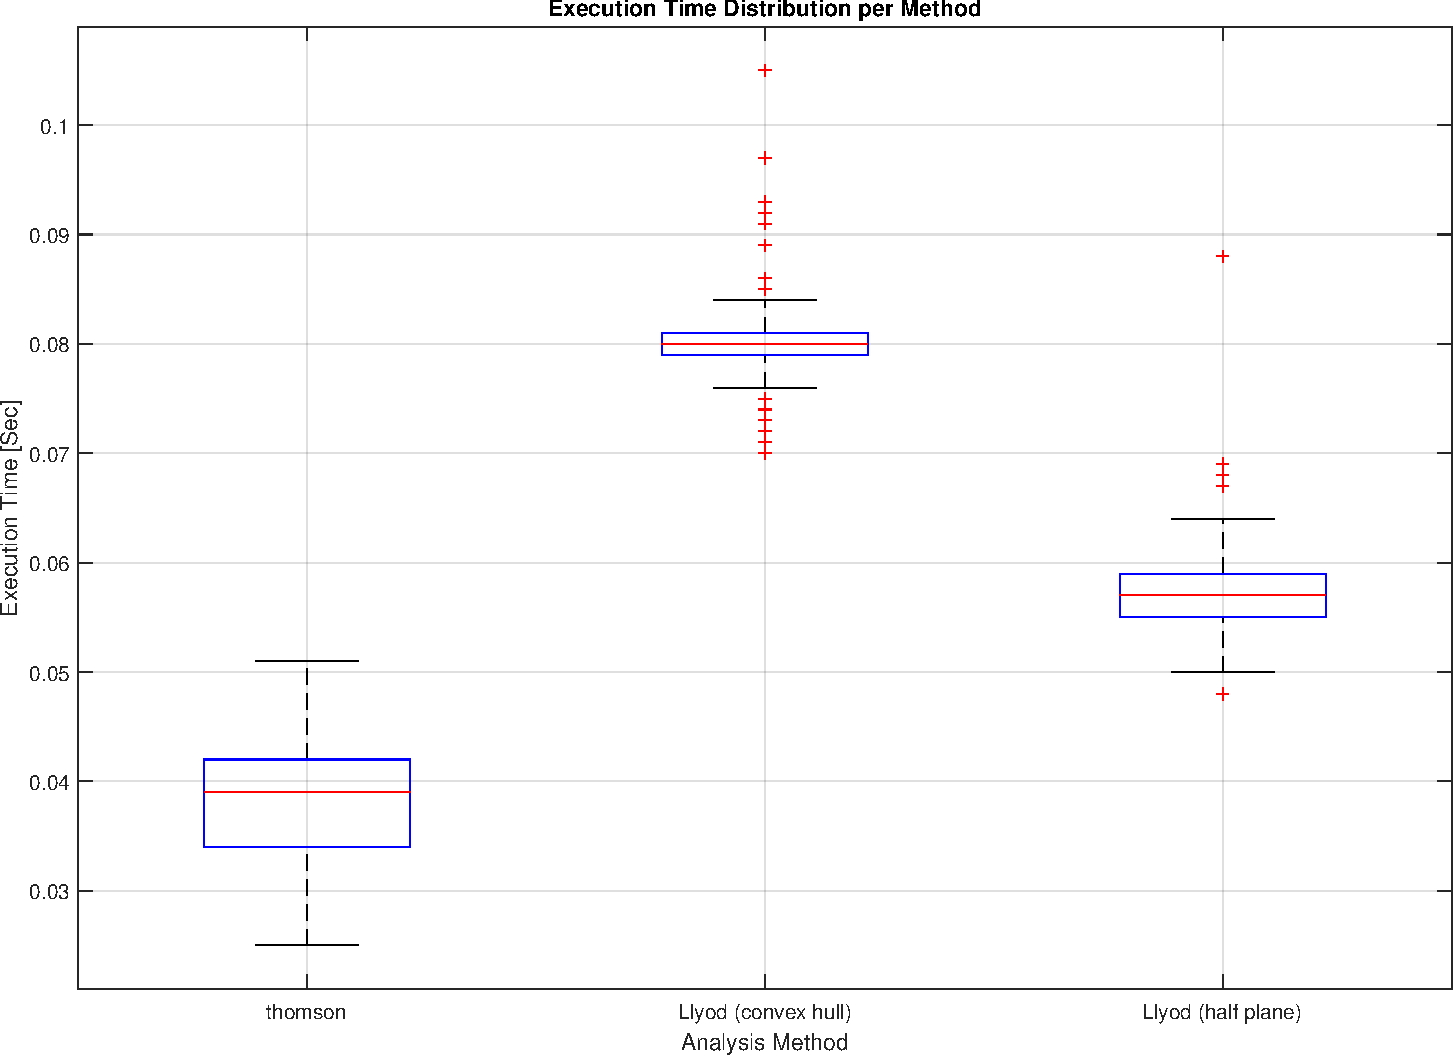
\includegraphics[width=0.85\textwidth]{5-Figures/Chapter5/iterative_comparing_methods_box_shape.pdf}
  \caption{Runtime  per iteration comparison of the different methods (100 iterations). Computer specification can be found at: \ref{appendix:Computer Specifications}}
  \label{fig.5:comparing_methods_box_shape}
\end{figure}

\begin{table}[htbp]
\caption{Runtime comparison of point sampling methods}
\label{tab.5:Runtime comparison of point sampling methods}
\centering
\begin{tabular}{l c c c c}
\hline
\textbf{Property}
& \makecell{\textbf{Thomson}}
& \makecell{\textbf{Lloyd (convex hull)}}
& \makecell{\textbf{Lloyd (half plane)}}\\
\hline
\makecell{Parameters}
& \makecell{MaxIter=100,\\ Seed=0}
& \makecell{--} 
& \makecell{--} \\

\makecell{Number of points}
& \makecell{1001}
& \makecell{1001} 
& \makecell{30} \\

\makecell{Mean runtime\\ (s)}
& \makecell{0.0752}
& \makecell{0.0806} 
& \makecell{0.0574} \\

\makecell{Std. deviation\\ $\sigma$ (s)}
& \makecell{0.0054}
& \makecell{0.0051} 
& \makecell{0.0048} \\
\hline
\end{tabular}
\end{table}

Although the per-iteration runtimes shown in Figure~\ref{fig.5:comparing_methods_box_shape} and Table~\ref{tab.5:Runtime comparison of point sampling methods} suggest comparable computational costs across all methods, these results must be interpreted with caution. Different implementations of Lloyd's algorithm—particularly in how the Voronoi regions, areas, and centroids are computed—can lead to significantly different execution times.

For instance, the half-plane implementation may appear faster than the convex hull approach; however, this is largely due to the difference in the number of points used in the calculations. When evaluated with 1001 points, the half-plane implementation required approximately 855.8370 seconds (14.2639 minutes) per iteration. While this may initially suggest that the method is impractical, it is important to recognize that it involves trade-offs when compared to the convex hull implementation.

A direct comparison of computation times may therefore be biased by implementation details. For this reason, both theoretical computational complexity and prior comparisons are considered when selecting the most appropriate method.

In practice, Lloyd's algorithm typically converges to a sufficiently uniform distribution after a relatively small number of iterations, as it is often terminated once the configuration meets application-specific requirements. In contrast, global energy minimization approaches, such as the Thomson formulation, require solving a highly coupled optimization problem in which all points interact. This results in significantly higher computational cost and slower convergence, particularly as the number of points increases. Formally, the computational complexity of the Thomson formulation is $\mathcal{O}(n^2)$ due to pairwise interactions. Lloyd's algorithm, when implemented using convex hulls, has complexity $\mathcal{O}(kn)$, where $k$ is the number of edges associated with each point and $n$ is the total number of points~\cite{giffonQuicKmeansAcceleratingInference2021}. In contrast, the half-plane implementation of Lloyd's algorithm also exhibits $\mathcal{O}(n^2)$ complexity~\cite{fanHalfPlaneVoronoiDiagram2011}. Once again this may induce the idea that Lloyd method using a convex hull is faster and the other two methods should take the same amount of time, but as has been previously mentioned the Lloyd half plane method took 14.2639 minutes to run a single iteration, this comes to the implementation of the method it self, at the moment optimization is not a priority being only method comparison desired so a very suboptimal implementation of Lloyd half plane method has been done. In particular, the developed half-plane implementation of Lloyd's algorithm is significantly slower due to its reliance on the MATLAB function \cite{MATLAB_sphere} from \(\text{MATLAB}^\text{\textregistered}\)~\cite{MATLAB:R2024a}. As described in Section~\ref{sec.3:Iterative computation agent spacing on the two-sphere}, Voronoi regions are obtained by intersecting the spherical manifold with planes defined at the midpoints of geodesic curves. This approach is computationally expensive, as representing the sphere with sufficient resolution requires at least as many triangular surface elements as the number of points (e.g., at least 1001 elements for 1001 points) to ensure that the Voronoi regions are non-empty.

In Figure~\ref{fig.5:run_time_comparison} it is possible to see all three methods ran 100 times, having the average time of computation of the first 100 iteration of simulation for 30 agents. This was chosen a way to clean the ambiguity of the previous paragraph while being a realistic use case for encirclement. In this figure it is much more clear to see the execution time of each method for the used implementation, which is detailed in Section~\ref{sec.3:Iterative computation agent spacing on the two-sphere}. From Figure~\ref{fig.5:results_afete_100_iter} is is possible to see that indeed the Thomson method has a much slower evolution to a almost even spacing of points, since both implementation of Llyod's Algorithm have stabilized but Thomson's method has not. 

\begin{figure}[htbp]
  \centering
  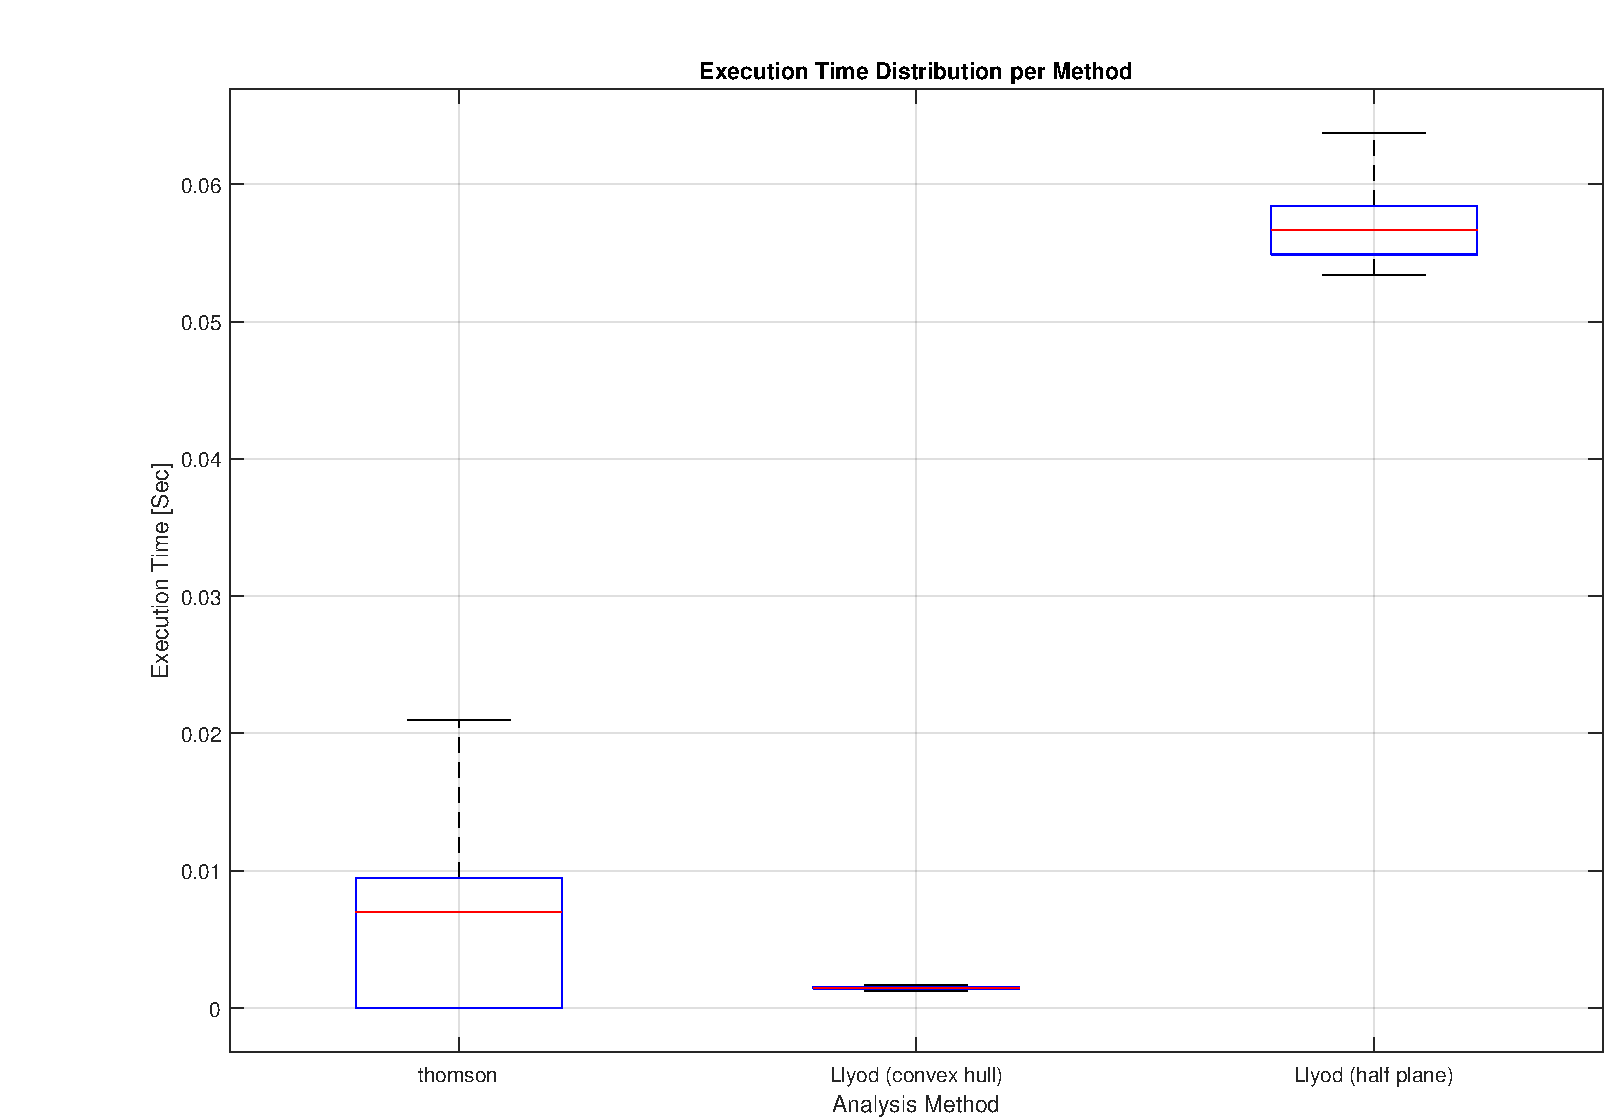
\includegraphics[width=0.85\textwidth]{5-Figures/Chapter5/iterative_run_comparing_methods_box_shape.pdf}
  \caption{Run time of 100 simulations of 100 iterations each}
  \label{fig.5:run_time_comparison}
\end{figure}


\begin{figure}[htbp]
    \centering
    \subfloat[Thomson]{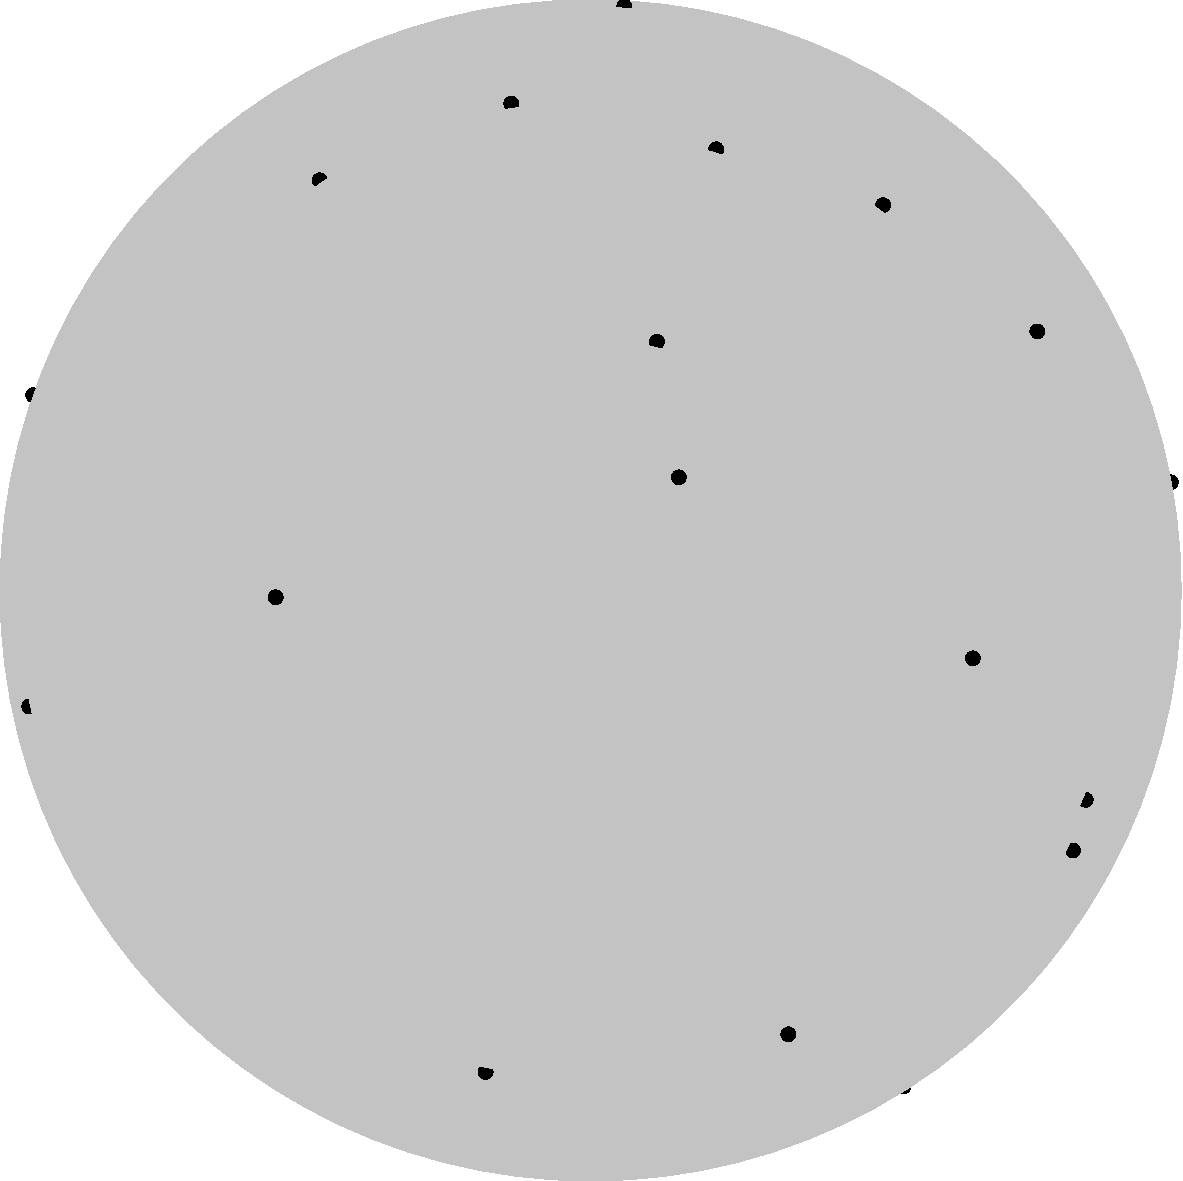
\includegraphics[width=3cm]{5-Figures/Chapter5/Comparisions/thomson_normal_100_iter.pdf}}\hfil
    \subfloat[convex hull]{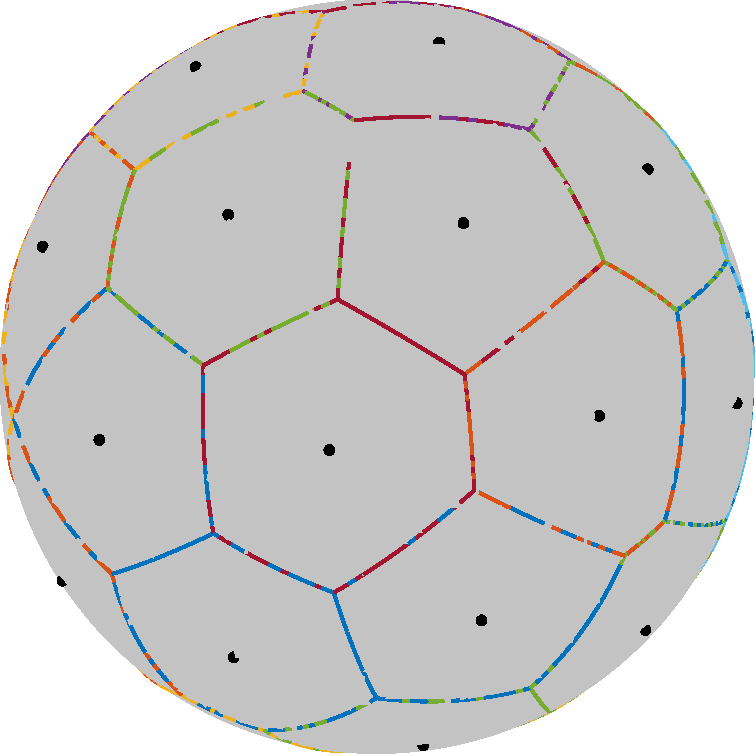
\includegraphics[width=3cm]{5-Figures/Chapter5/Comparisions/Lloyd_convex_hull_normal_100_iter.pdf}}\hfil
    \subfloat[half plane]{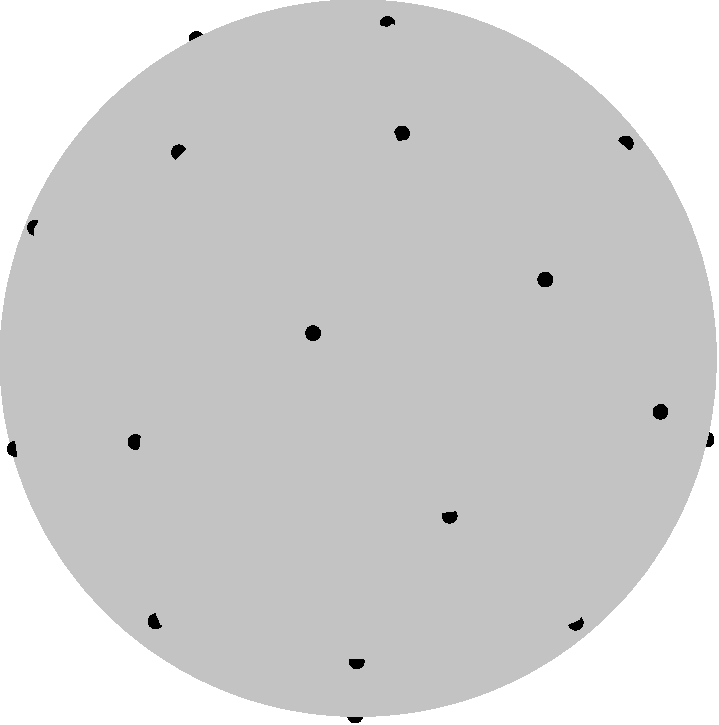
\includegraphics[width=3cm]{5-Figures/Chapter5/Comparisions/Lloyd_half_plane_normal_100_iter.pdf}}
    \caption{Different methods results after 100 iterations}
    \label{fig.5:results_afete_100_iter}
\end{figure}

From the above analysis it is concluded that complete system simulations of the complete control architecture is to be tested for both Lloyd's implementation methods developed, since both have their benefits, being the convex hull much faster but prone to errors based on the use of the Matlab function convex hull that creates flat triangular surfaces and the projection of said surfaces to the sphere may cause the system to collapse and the half plane method that seams to work independently of the number of agents or initial position.

\section{Control architecture}

The control architecture of the Decentralized version of the system is very similar to the final version of the centralized one. There are two major differences, the use of the Lloyd's Algorithm instead of the fibonacci lattice due to no agent knowing the total number of agents in the formation nor their position as well as the use of a small world network previously mentioned in Section~\ref{sec.3:Network topologies}. With the use of this two additions it is possible for the system to be completely decentralized. In Figure~\ref{fig.5:Controller architecture} its possible to see the complete system architecture, note that the only input of the system is the target position.

\begin{figure}[htbp]
  \centering
  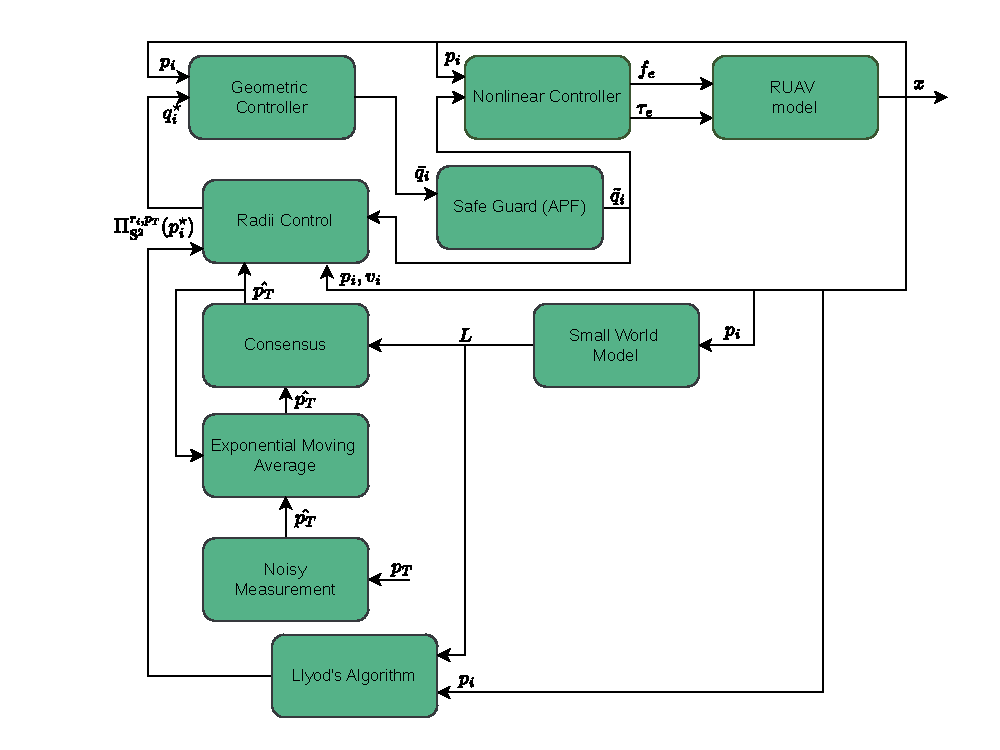
\includegraphics[width=0.85\textwidth]{5-Figures/Chapter5/controller_architecture/decentralized_complete_controller_architecture.drawio.pdf}
  \caption{Controller architecture}
  \label{fig.5:Controller architecture}
\end{figure}

\section{Dynamic Network}

The concept of a small-world network was previously introduced in Section~\ref{sec.3:Network topologies}. In the present context, the network is recomputed at every time step, ensuring that connections between agents reflect their current spatial configuration. In particular, each agent connects to its current set of nearest neighbors, rather than maintaining links from a potentially outdated network topology resulting from agent motion.

However, methods based on a fixed number of $k$-nearest neighbors or on distance-based communication thresholds present important limitations. These approaches rely on static parameters that may not be suitable for dynamic scenarios. For instance, in the case of $k$-nearest neighbors, imposing a fixed number of connections can be overly restrictive, failing to capture all relevant neighboring relationships. As illustrated in Figure~\ref{fig.5:KNN_problems}, some edges that should define the natural boundaries between regions are neglected. This leads to inconsistencies, such as regions being effectively counted multiple times due to missing adjacency relationships. If a high value of $k$ is considered then some connections will exist and not be necessary becoming unnecessary calculations that are overhead for most agents.  

Similarly, distance-based communication models, where agents connect if they lie within a fixed radius, are also problematic. As agents move, maintaining connectivity may require dynamically increasing the communication radius. Otherwise, agents may lose connectivity entirely when their mutual distances exceed the predefined threshold, potentially resulting in a disconnected network.

\begin{figure}[htbp]
  \centering
  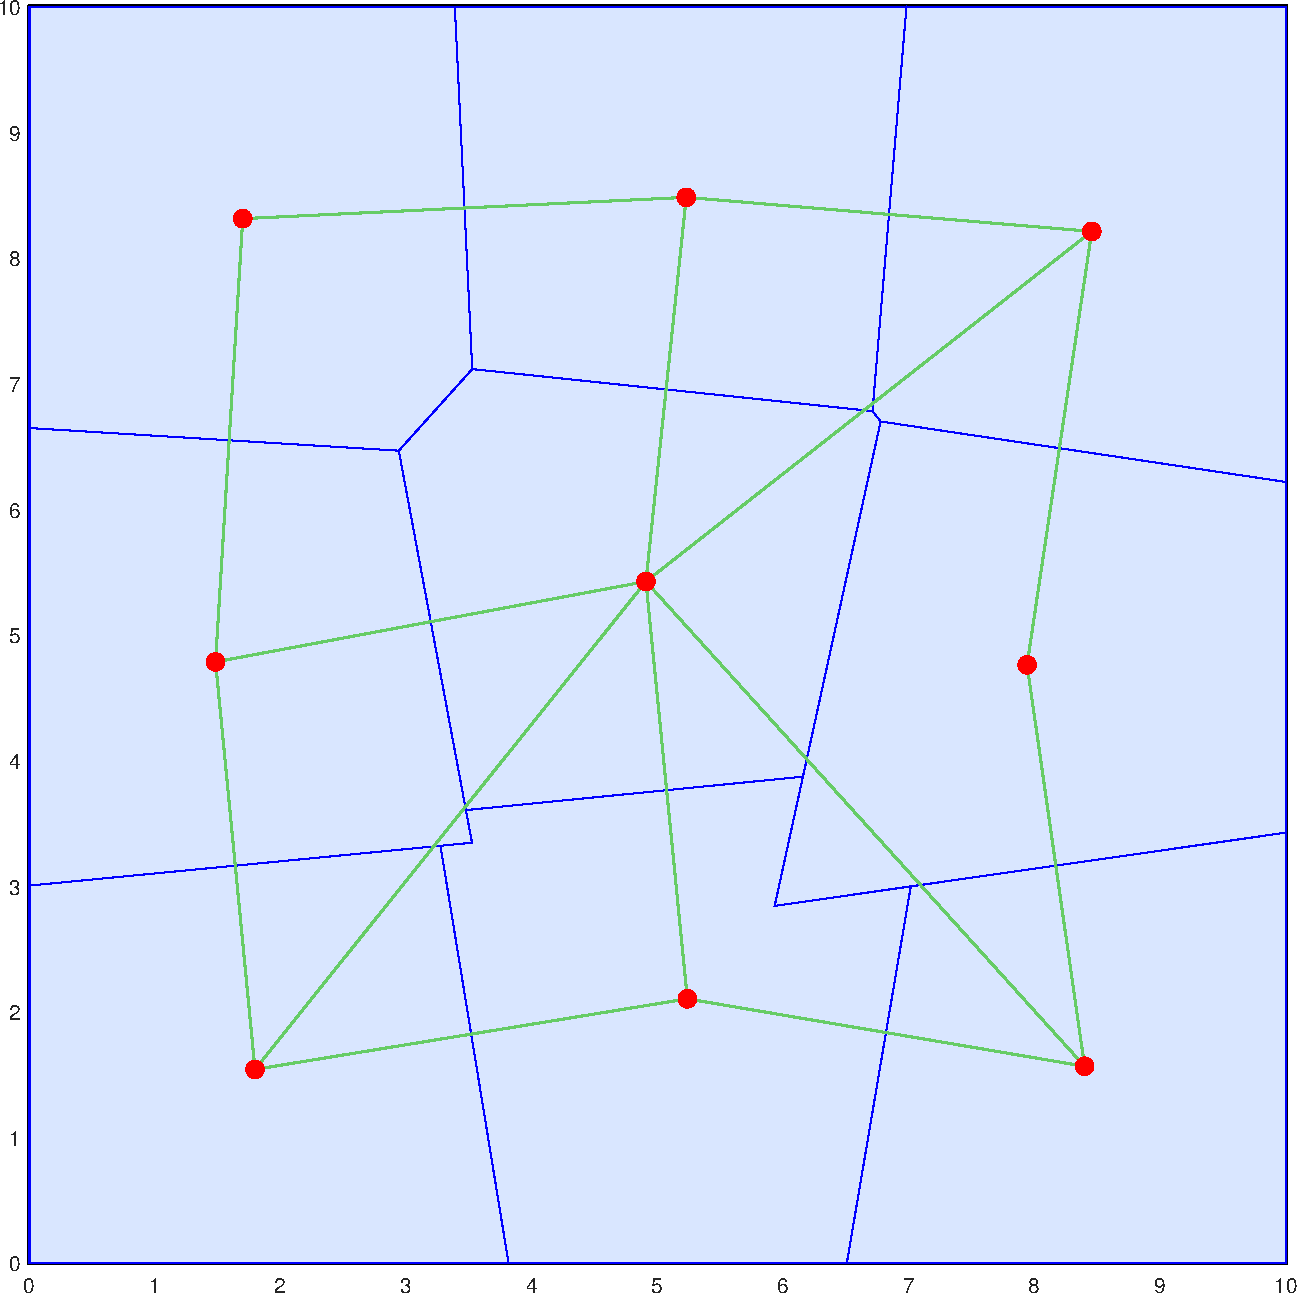
\includegraphics[width=0.85\textwidth]{5-Figures/Chapter5/Networks/KNN_problems.pdf}
  \caption{N-nearest neighbor faults}
  \label{fig.5:KNN_problems}
\end{figure}

To address these issues, the communication graph is instead defined using the Delaunay triangulation. This structure is already computed as part of Lloyd's algorithm and the associated Voronoi diagram, making it a natural and computationally efficient choice. The Delaunay triangulation provides an adaptive and topology-preserving representation of agent connectivity, ensuring that neighboring relationships are consistently maintained as agents move. Figure~\ref{fig.5:Delaunay Triangulation} illustrates the resulting triangulation and the corresponding communication links between agents.

\begin{figure}[htbp]
  \centering
  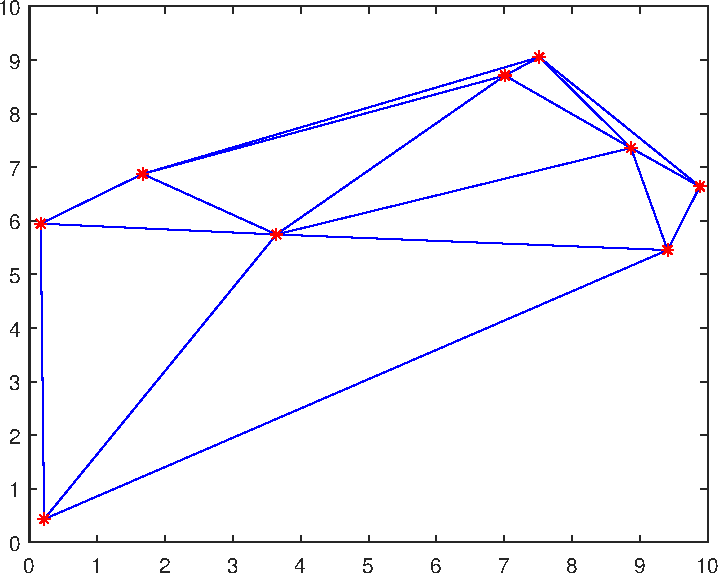
\includegraphics[width=0.85\textwidth]{5-Figures/Chapter5/Networks/delaunay_triangulation.pdf}
  \caption{Delaunay Triangulation in $\mathbb{R}^2$}
  \label{fig.5:Delaunay Triangulation}
\end{figure}

\section{Voronoi-Based Decentralized Update}

The decentralized redistribution of agents over a spherical surface is achieved through a local Voronoi-based update rule. This approach is inspired by the classical Lloyd algorithm, but adapted to operate under decentralized conditions.

In this formulation, each agent constructs a local Voronoi diagram considering only its own position and those of its immediate neighbors. Unlike the centralized Lloyd algorithm, where all Voronoi cells are computed globally, each agent evaluates only its own Voronoi region. The centroid of this local cell is then computed, and the agent updates its position accordingly. Importantly, from the perspective of each agent, it is the only entity that moves, while neighboring agents are treated as static during the update step.

Although each agent operates using only local information, the collective behavior of the system approximates that of a fully centralized implementation. That is, if all agents simultaneously apply this local rule, the resulting motion is equivalent to each agent moving toward the centroid of its corresponding Voronoi cell in the global tessellation.

A key advantage of this method is that it requires only local communication. Each agent needs access solely to the positions of its neighboring agents, and no global knowledge such as the total number of agents in the system is required. This makes the approach scalable and well-suited for distributed implementations.

However, this method assumes that the domain in which the agents operate is bounded. In Euclidean space ($\mathbb{R}^2$), this corresponds to environments with well-defined boundaries. In the case of a spherical surface, the domain is inherently bounded by the geometry of the sphere itself, which naturally constrains the Voronoi regions. The implementation of this methods is as follows, for a given agent $i$, a local set of points is first constructed as
\begin{equation}
\mathcal{P}_i = \left\{ \mathbf{q}_i \right\} \cup \left\{ \mathbf{q}_j \mid j \in \mathcal{N}_i \right\},
\end{equation}
where $\mathbf{q}_i \in \mathbb{R}^3$ is the desired position of agent $i$ and $\mathcal{N}_i$ denotes its set of neighbors, obtained from the  delaunay triangulation. These points are projected onto the unit sphere according to

\begin{equation*}
\hat{\mathbf{p}} = \Pi_{\Gamma^2}^{1,0} \mathcal{P}
\end{equation*}

The convex hull of the normalized set $\hat{\mathcal{P}}_i$ is then computed using the internal \(\text{MATLAB}^\text{\textregistered}\) \cite{MATLAB:R2024a} function \cite{MATLAB_convhull}, and only the triangular faces that include agent $i$ are retained. For each triangular face defined by three points $\hat{\mathbf{p}}_a$, $\hat{\mathbf{p}}_b$, and $\hat{\mathbf{p}}_c$, a candidate Voronoi vertex is obtained as the normalized cross product
\begin{equation}
\mathbf{v} = \frac{(\hat{\mathbf{p}}_b - \hat{\mathbf{p}}_a) \times (\hat{\mathbf{p}}_c - \hat{\mathbf{p}}_a)}{\|(\hat{\mathbf{p}}_b - \hat{\mathbf{p}}_a) \times (\hat{\mathbf{p}}_c - \hat{\mathbf{p}}_a)\|}.
\end{equation}
To ensure consistent orientation, each vertex is aligned with the outward radial direction of agent $i$:
\begin{equation}
\mathbf{v} \leftarrow 
\begin{cases}
\mathbf{v}, & \text{if } \mathbf{v} \cdot \hat{\mathbf{q}}_i > 0, \\
-\mathbf{v}, & \text{otherwise}.
\end{cases}
\end{equation}

The resulting set of Voronoi vertices is then projected onto a local tangent plane for ordering. Let $\mathbf{V} \in \mathbb{R}^{m \times 3}$ be the matrix of vertices and $\hat{\mathbf{q}}_i$ the agent position. A local 2D parametrization is obtained via singular value decomposition:
\begin{equation}
\mathbf{V} - \hat{\mathbf{q}}_i = \mathbf{U} \mathbf{\Sigma} \mathbf{W}^\top,
\end{equation}
and the projection onto the first two principal directions yields
\begin{equation}
\mathbf{p}_k = (\mathbf{v}_k - \hat{\mathbf{q}}_i)\mathbf{W}_{(:,1:2)}.
\end{equation}
The vertices are then ordered according to their angular coordinate
\begin{equation}
\theta_k = \mathrm{atan2}(p_{k,2}, p_{k,1}).
\end{equation}

The centroid of the spherical Voronoi region is approximated by decomposing it into spherical triangles. For a triangle defined by unit vectors $\mathbf{a}$, $\mathbf{b}$, and $\mathbf{c}$ on the sphere, the side lengths are first computed using angular distances
\begin{equation}
\alpha = \arccos(\mathbf{b} \cdot \mathbf{c}), \quad
\beta  = \arccos(\mathbf{a} \cdot \mathbf{c}), \quad
\gamma = \arccos(\mathbf{a} \cdot \mathbf{b}).
\end{equation}
The area of the spherical triangle is then computed using L'Huilier's theorem \cite{L_Huilier1809} as
\begin{equation}
A = 4 \arctan \left( \sqrt{
\tan\left(\frac{s}{2}\right)
\tan\left(\frac{s-\alpha}{2}\right)
\tan\left(\frac{s-\beta}{2}\right)
\tan\left(\frac{s-\gamma}{2}\right)
} \right).
\end{equation}
where
\begin{equation}
s = \frac{\alpha + \beta + \gamma}{2}
\end{equation}
is the semi-perimeter. 

The centroid of each spherical triangle is approximated by the normalized sum of its vertices,
\begin{equation}
\mathbf{g} = \frac{\mathbf{a} + \mathbf{b} + \mathbf{c}}{\|\mathbf{a} + \mathbf{b} + \mathbf{c}\|},
\end{equation}
and the overall Voronoi centroid is obtained as the area-weighted average of these triangle centroids.
\begin{equation}
\mathbf{g}_i = \frac{\sum_{k} A_k \mathbf{g}_k}{\left\|\sum_{k} A_k \mathbf{g}_k \right\|}.
\end{equation}

Finally, the updated desired position of the agent is computed by projecting this centroid back onto the sphere:
\begin{equation*}
\gls{q_i_desired} = \Pi_{\Gamma^2}^{r_i,P_T} \mathbf{g}_i
\end{equation*}

\section{Simulation Results (convex hull)}

The system was evaluated using a total of 12 agents performing the encirclement of a moving target. The results are presented in Figures \ref{fig.5:decentralized_results_drone_1} and \ref{fig.5:lyapunov_solution_t_0.5}--\ref{fig.5:lyapunov_solution_t_30}. The parameters used are identical to those of the centralized system and are listed in Tables~\ref{tab.4:all_params} and \ref{tab.4:Drone_positions}. The reference target position, $\gls{target_pos}^\star$, was chosen to be the same as in the centralized system experiments.

\begin{figure}[htbp]
    \centering
    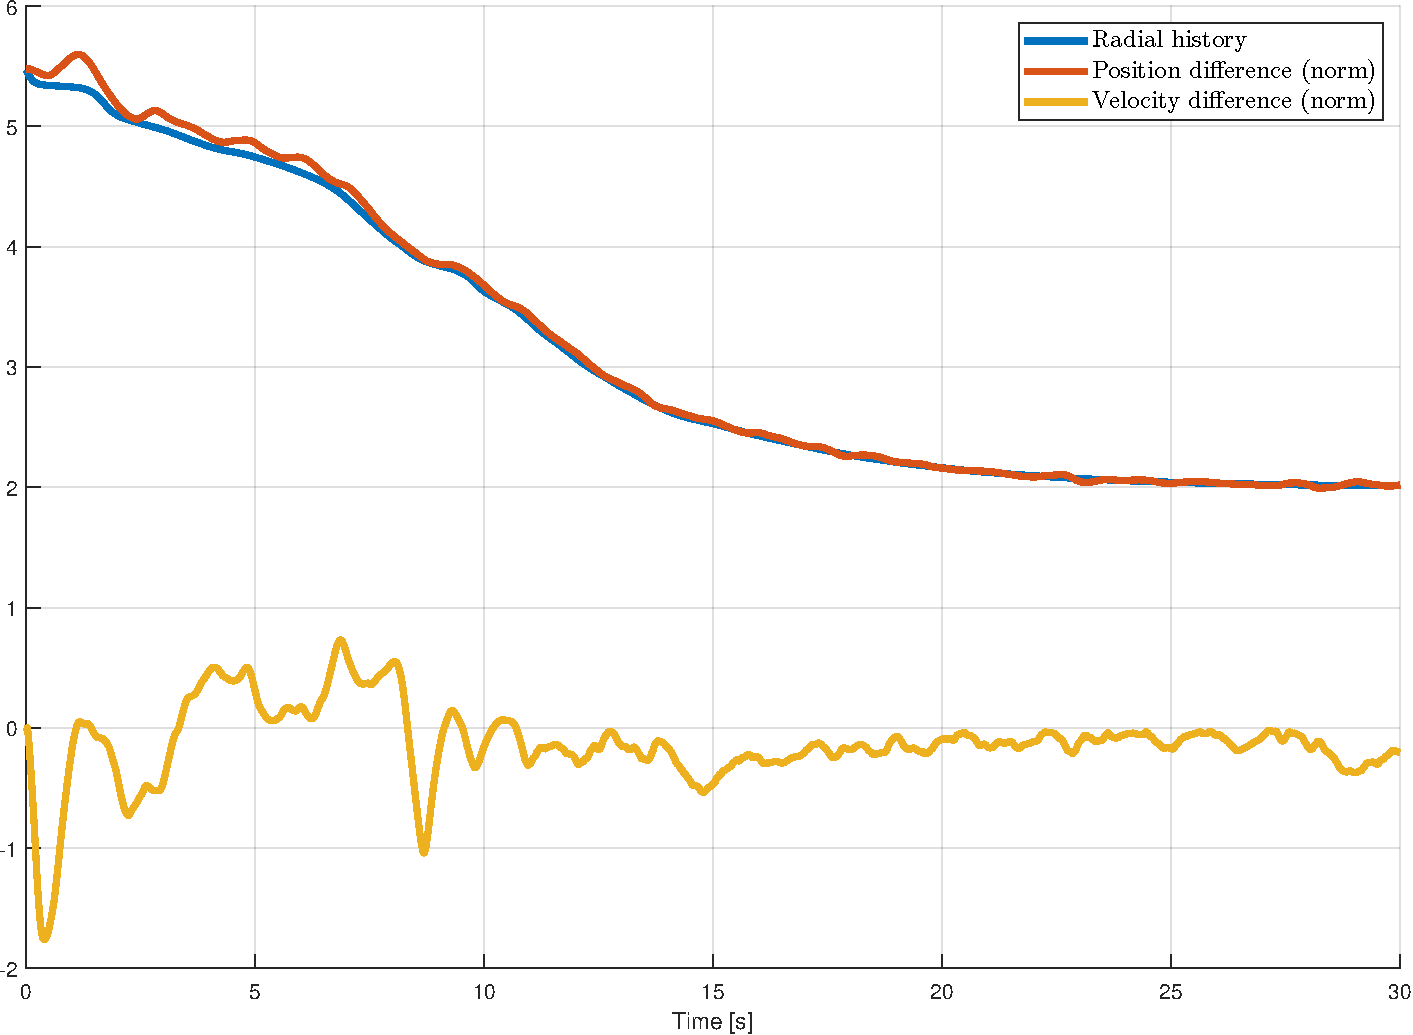
\includegraphics[width=0.85\columnwidth]{5-Figures/Chapter5/Simulations/decentralized_results_drone_1.pdf}
    \caption{Distance and velocity between drone 1 and a moving target}
    \label{fig.5:decentralized_results_drone_1}
\end{figure}

\begin{figure}[htbp]
    \centering
    \subfloat[$t=0.5~\mathrm{s}$]{%
        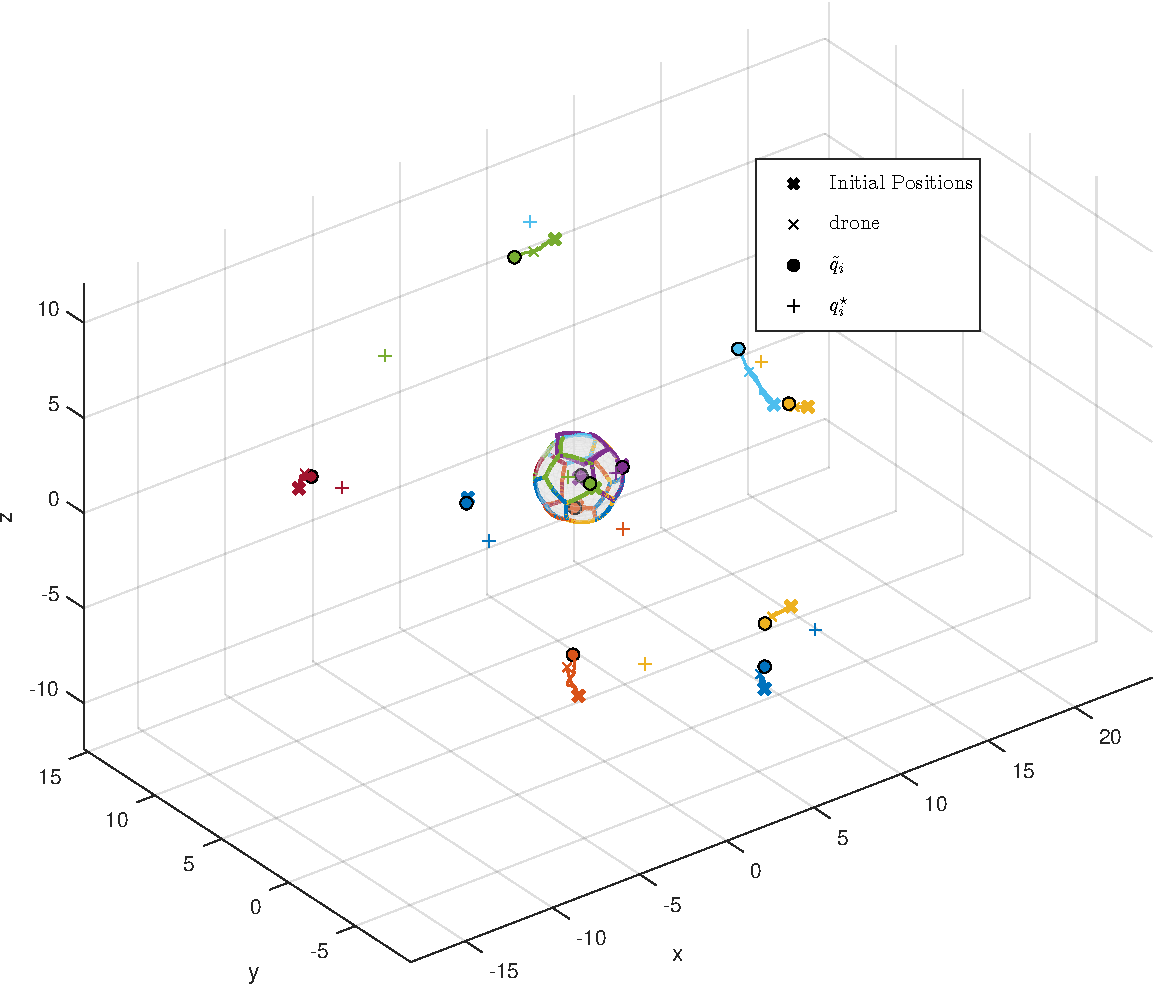
\includegraphics[width=0.5\columnwidth]{5-Figures/Chapter5/Simulations/decentralized_moving_t_0.5.pdf}\hfil
        \label{fig.5:lyapunov_solution_t_0.5}
    }
        \subfloat[$t=3~\mathrm{s}$]{%
        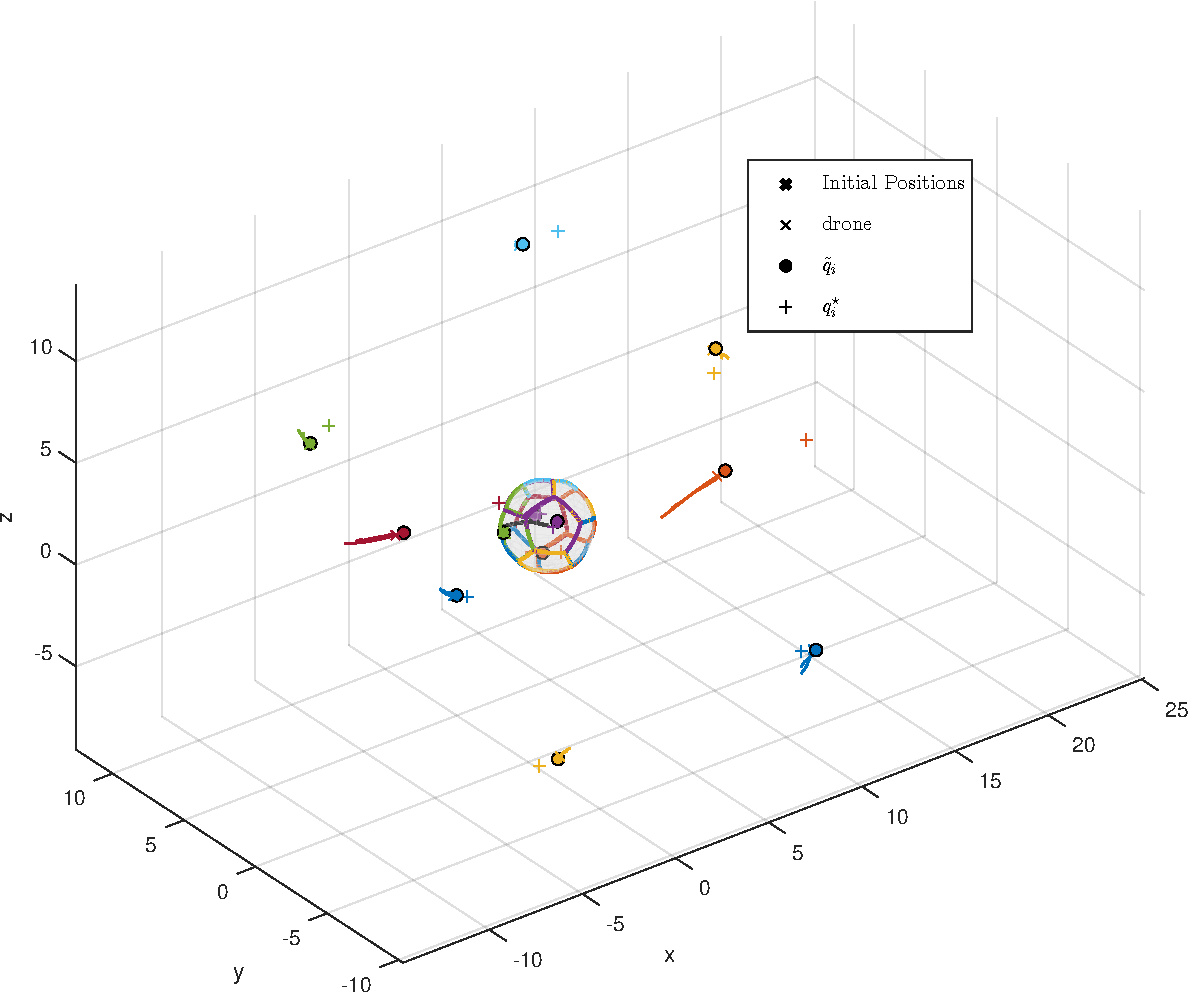
\includegraphics[width=0.5\columnwidth]{5-Figures/Chapter5/Simulations/decentralized_moving_t_3.pdf}\hfil
        \label{fig.5:lyapunov_solution_t_3}
    }\\
    \subfloat[$t=6~\mathrm{s}$]{%
        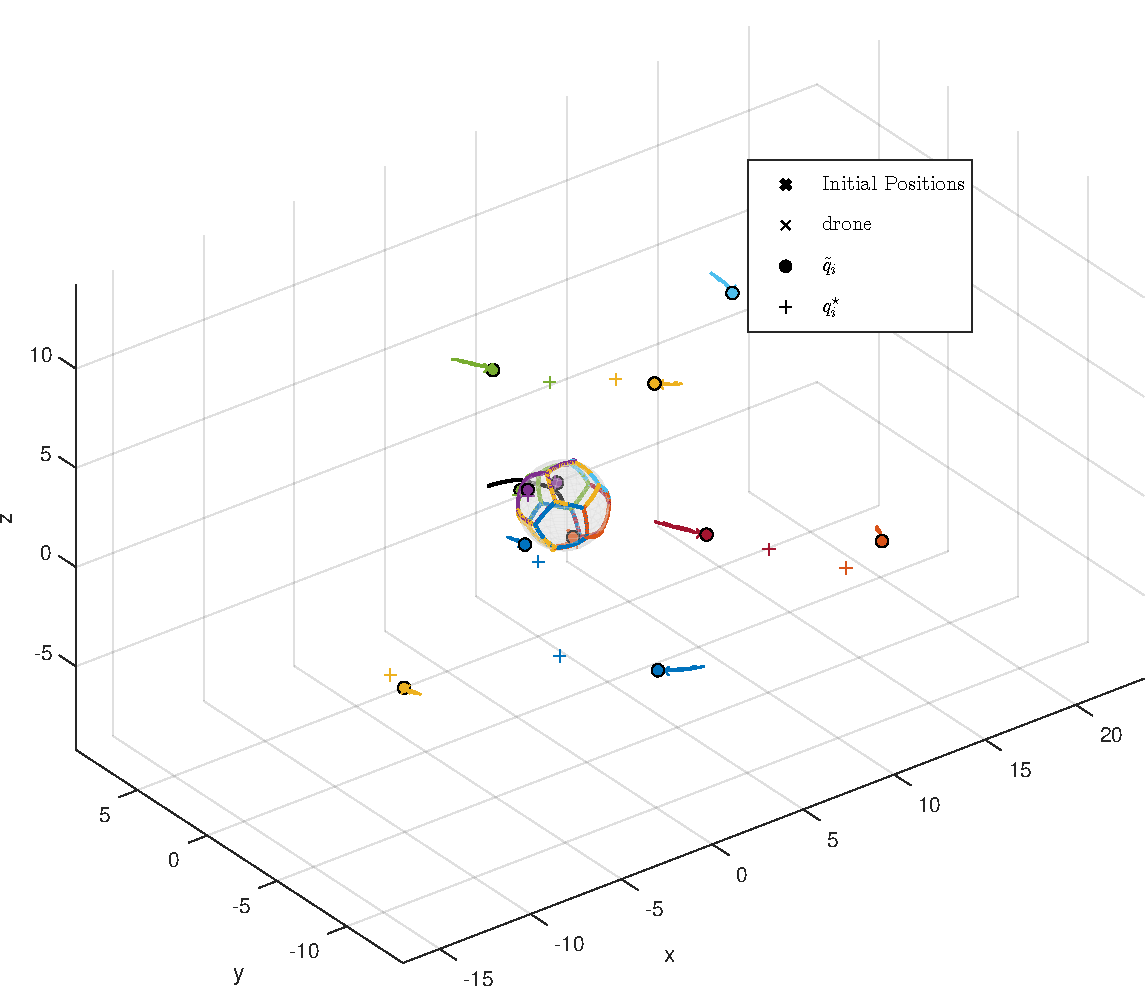
\includegraphics[width=0.5\columnwidth]{5-Figures/Chapter5/Simulations/decentralized_moving_t_6.pdf}\hfil
        \label{fig.5:lyapunov_solution_t_6}
    }
    \subfloat[$t=30~\mathrm{s}$]{%
        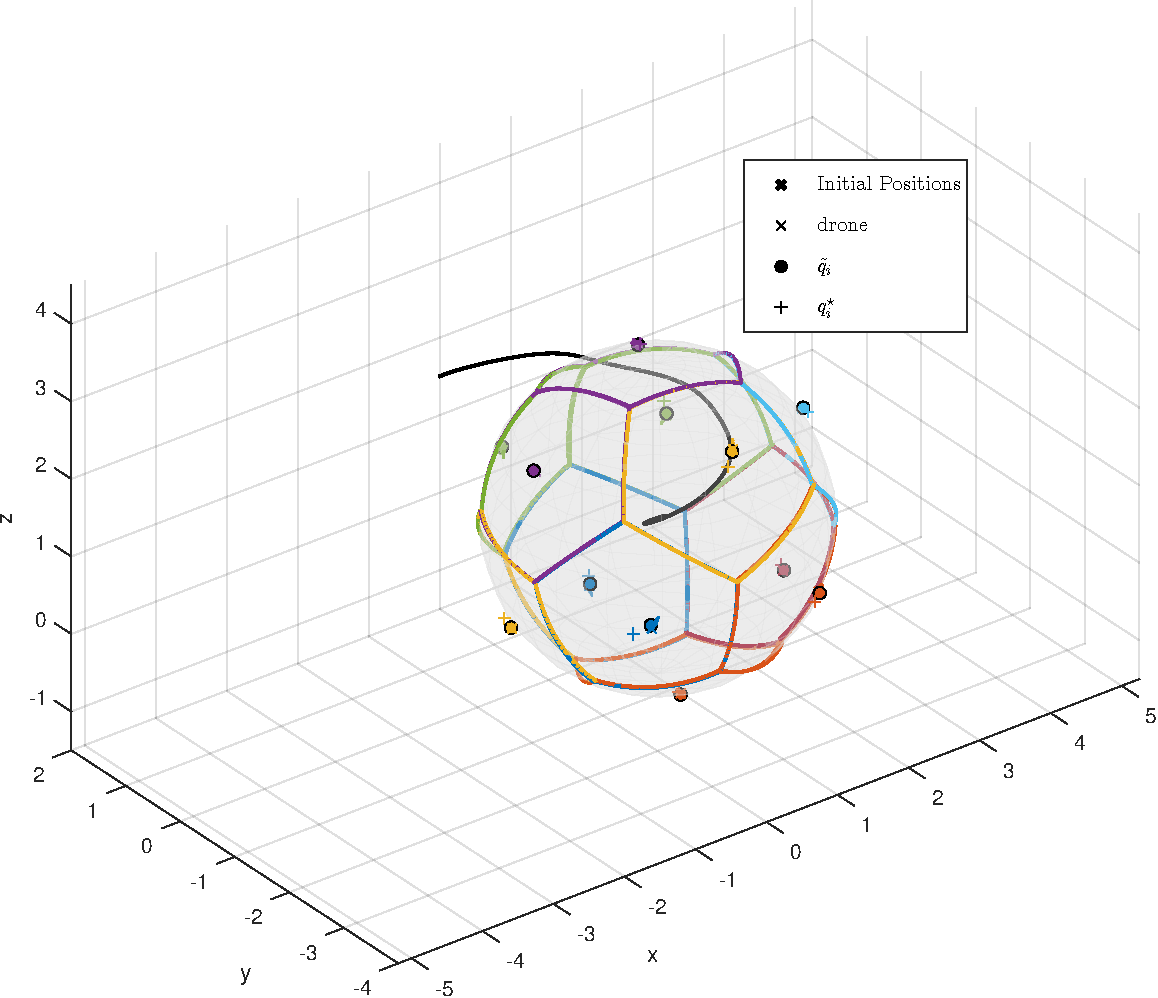
\includegraphics[width=0.5\columnwidth]{5-Figures/Chapter5/Simulations/decentralized_moving_t_30.pdf}
        \label{fig.5:lyapunov_solution_t_30}
    }
    \caption{Encirclement of a moving target using the Lyapunov-based control strategy for three drones at different time instants.}
    \label{fig.4:lyapunov_solution}
\end{figure}

\begin{figure}[htbp]
  \centering
  \subfloat[Normal]{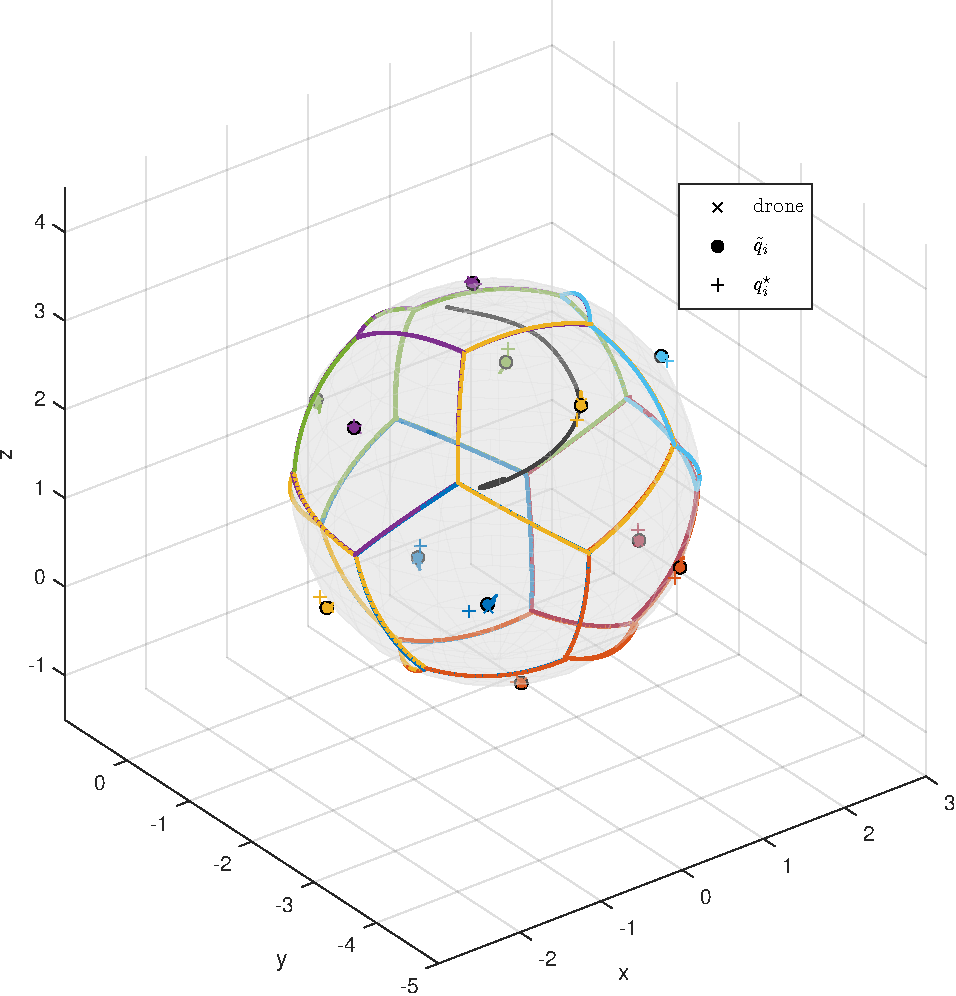
\includegraphics[width=5cm]{5-Figures/Chapter5/Simulations/decentralized_simulation_normal.pdf}}\hfil   
  \subfloat[Top]{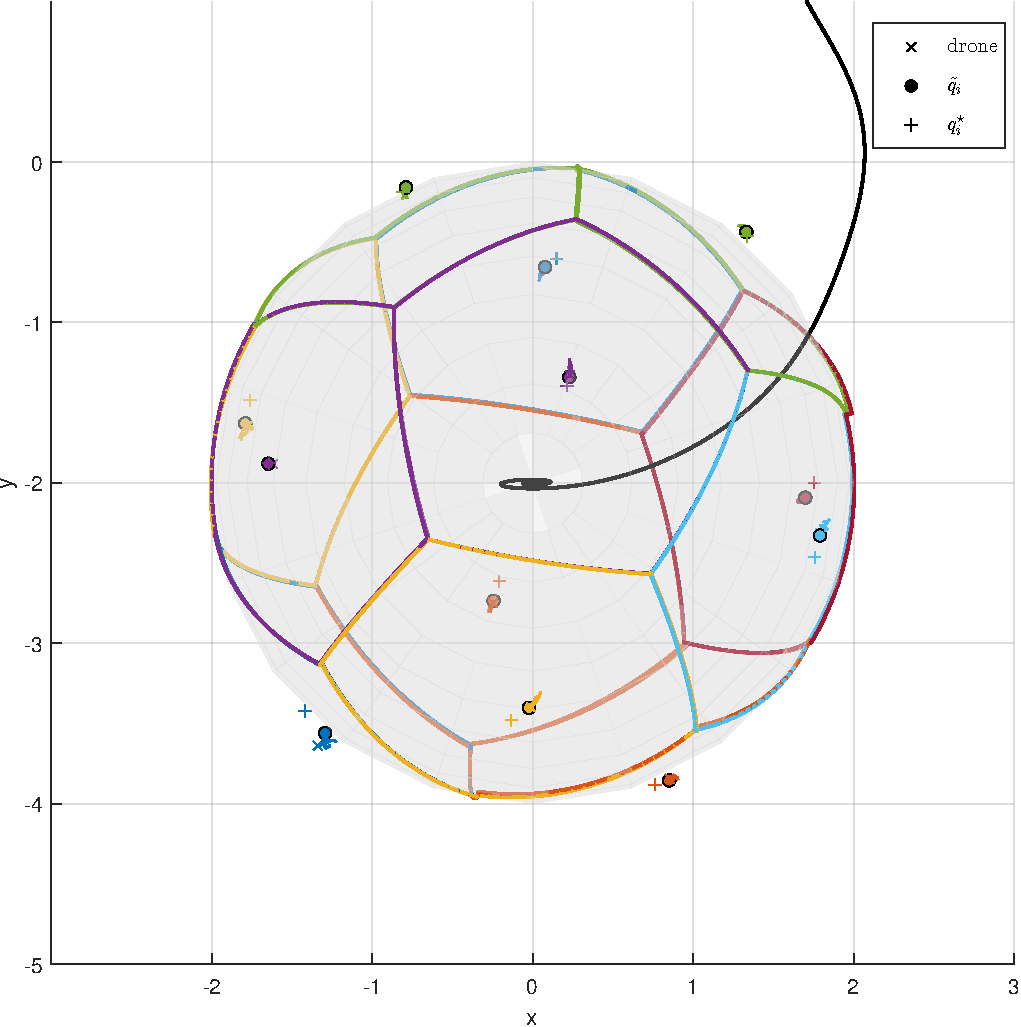
\includegraphics[width=5cm]{5-Figures/Chapter5/Simulations/decentralized_simulation_top.pdf}}\hfil
  \subfloat[Side]{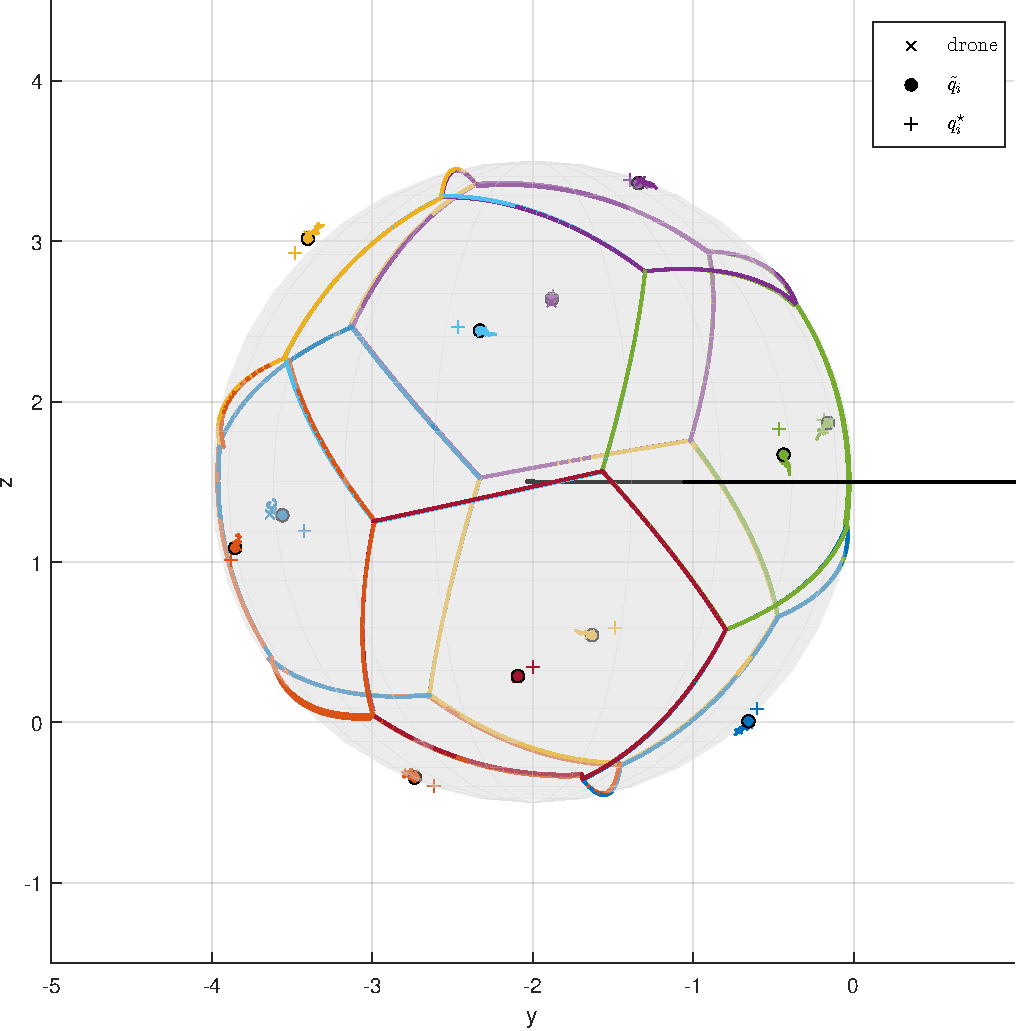
\includegraphics[width=5cm]{5-Figures/Chapter5/Simulations/decentralized_simulation_side.pdf}}
  \caption{3 views of final simulation drone positioning}
  \label{fig.3:fibonacci_lattice_demonstration}
\end{figure}

\section{Simulation Results (half plane)}